\begin{figure}[t]
\centering
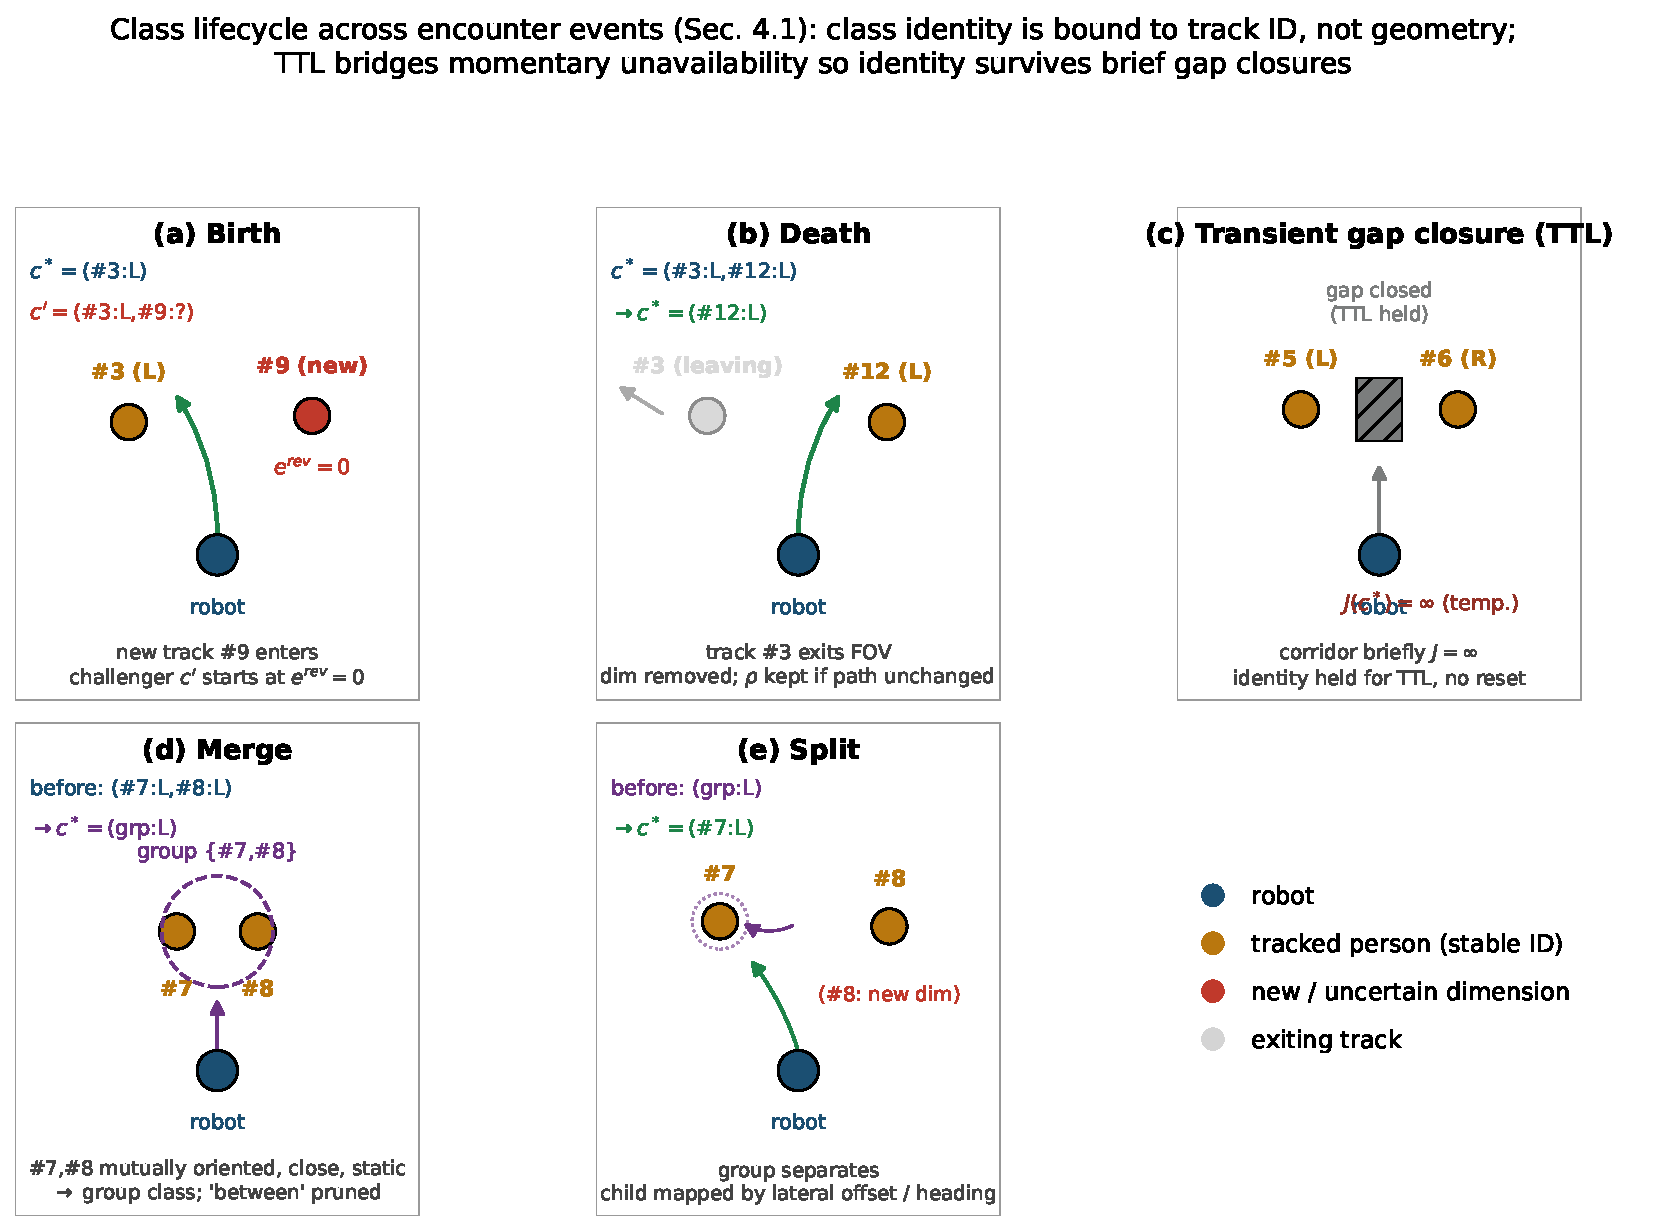
\includegraphics[width=\linewidth]{figures/fig_class_lifecycle.pdf}
\caption{\textbf{Lifecycle events of a topological class} (schematic). (a) Creation --- a new track appears as a challenger, starting from $\Erev=0$; (b) Extinction --- when a track leaves, the corresponding dimension is removed ($\rho$ is retained if the path is unchanged); (c) Temporary unavailability --- even when a corridor momentarily becomes $J=\infty$, identity is retained for a TTL to prevent a reset; (d) Merge --- two people judged by interaction cues (mutual orientation, proximity, low speed) merge into a single group class; (e) Split --- a group separates, mapped to the child class consistent with the robot's lateral offset and heading. Class identity is bound to human track IDs rather than geometry.}
\label{fig:lifecycle}
\end{figure}
